
% Default to the notebook output style

    


% Inherit from the specified cell style.




    
\documentclass[11pt]{article}

    
    
    \usepackage[T1]{fontenc}
    % Nicer default font (+ math font) than Computer Modern for most use cases
    \usepackage{mathpazo}

    % Basic figure setup, for now with no caption control since it's done
    % automatically by Pandoc (which extracts ![](path) syntax from Markdown).
    \usepackage{graphicx}
    % We will generate all images so they have a width \maxwidth. This means
    % that they will get their normal width if they fit onto the page, but
    % are scaled down if they would overflow the margins.
    \makeatletter
    \def\maxwidth{\ifdim\Gin@nat@width>\linewidth\linewidth
    \else\Gin@nat@width\fi}
    \makeatother
    \let\Oldincludegraphics\includegraphics
    % Set max figure width to be 80% of text width, for now hardcoded.
    \renewcommand{\includegraphics}[1]{\Oldincludegraphics[width=.8\maxwidth]{#1}}
    % Ensure that by default, figures have no caption (until we provide a
    % proper Figure object with a Caption API and a way to capture that
    % in the conversion process - todo).
    \usepackage{caption}
    \DeclareCaptionLabelFormat{nolabel}{}
    \captionsetup{labelformat=nolabel}

    \usepackage{adjustbox} % Used to constrain images to a maximum size 
    \usepackage{xcolor} % Allow colors to be defined
    \usepackage{enumerate} % Needed for markdown enumerations to work
    \usepackage{geometry} % Used to adjust the document margins
    \usepackage{amsmath} % Equations
    \usepackage{amssymb} % Equations
    \usepackage{textcomp} % defines textquotesingle
    % Hack from http://tex.stackexchange.com/a/47451/13684:
    \AtBeginDocument{%
        \def\PYZsq{\textquotesingle}% Upright quotes in Pygmentized code
    }
    \usepackage{upquote} % Upright quotes for verbatim code
    \usepackage{eurosym} % defines \euro
    \usepackage[mathletters]{ucs} % Extended unicode (utf-8) support
    \usepackage[utf8x]{inputenc} % Allow utf-8 characters in the tex document
    \usepackage{fancyvrb} % verbatim replacement that allows latex
    \usepackage{grffile} % extends the file name processing of package graphics 
                         % to support a larger range 
    % The hyperref package gives us a pdf with properly built
    % internal navigation ('pdf bookmarks' for the table of contents,
    % internal cross-reference links, web links for URLs, etc.)
    \usepackage{hyperref}
    \usepackage{longtable} % longtable support required by pandoc >1.10
    \usepackage{booktabs}  % table support for pandoc > 1.12.2
    \usepackage[inline]{enumitem} % IRkernel/repr support (it uses the enumerate* environment)
    \usepackage[normalem]{ulem} % ulem is needed to support strikethroughs (\sout)
                                % normalem makes italics be italics, not underlines
    \usepackage{mathrsfs}
    

    
    
    % Colors for the hyperref package
    \definecolor{urlcolor}{rgb}{0,.145,.698}
    \definecolor{linkcolor}{rgb}{.71,0.21,0.01}
    \definecolor{citecolor}{rgb}{.12,.54,.11}

    % ANSI colors
    \definecolor{ansi-black}{HTML}{3E424D}
    \definecolor{ansi-black-intense}{HTML}{282C36}
    \definecolor{ansi-red}{HTML}{E75C58}
    \definecolor{ansi-red-intense}{HTML}{B22B31}
    \definecolor{ansi-green}{HTML}{00A250}
    \definecolor{ansi-green-intense}{HTML}{007427}
    \definecolor{ansi-yellow}{HTML}{DDB62B}
    \definecolor{ansi-yellow-intense}{HTML}{B27D12}
    \definecolor{ansi-blue}{HTML}{208FFB}
    \definecolor{ansi-blue-intense}{HTML}{0065CA}
    \definecolor{ansi-magenta}{HTML}{D160C4}
    \definecolor{ansi-magenta-intense}{HTML}{A03196}
    \definecolor{ansi-cyan}{HTML}{60C6C8}
    \definecolor{ansi-cyan-intense}{HTML}{258F8F}
    \definecolor{ansi-white}{HTML}{C5C1B4}
    \definecolor{ansi-white-intense}{HTML}{A1A6B2}
    \definecolor{ansi-default-inverse-fg}{HTML}{FFFFFF}
    \definecolor{ansi-default-inverse-bg}{HTML}{000000}

    % commands and environments needed by pandoc snippets
    % extracted from the output of `pandoc -s`
    \providecommand{\tightlist}{%
      \setlength{\itemsep}{0pt}\setlength{\parskip}{0pt}}
    \DefineVerbatimEnvironment{Highlighting}{Verbatim}{commandchars=\\\{\}}
    % Add ',fontsize=\small' for more characters per line
    \newenvironment{Shaded}{}{}
    \newcommand{\KeywordTok}[1]{\textcolor[rgb]{0.00,0.44,0.13}{\textbf{{#1}}}}
    \newcommand{\DataTypeTok}[1]{\textcolor[rgb]{0.56,0.13,0.00}{{#1}}}
    \newcommand{\DecValTok}[1]{\textcolor[rgb]{0.25,0.63,0.44}{{#1}}}
    \newcommand{\BaseNTok}[1]{\textcolor[rgb]{0.25,0.63,0.44}{{#1}}}
    \newcommand{\FloatTok}[1]{\textcolor[rgb]{0.25,0.63,0.44}{{#1}}}
    \newcommand{\CharTok}[1]{\textcolor[rgb]{0.25,0.44,0.63}{{#1}}}
    \newcommand{\StringTok}[1]{\textcolor[rgb]{0.25,0.44,0.63}{{#1}}}
    \newcommand{\CommentTok}[1]{\textcolor[rgb]{0.38,0.63,0.69}{\textit{{#1}}}}
    \newcommand{\OtherTok}[1]{\textcolor[rgb]{0.00,0.44,0.13}{{#1}}}
    \newcommand{\AlertTok}[1]{\textcolor[rgb]{1.00,0.00,0.00}{\textbf{{#1}}}}
    \newcommand{\FunctionTok}[1]{\textcolor[rgb]{0.02,0.16,0.49}{{#1}}}
    \newcommand{\RegionMarkerTok}[1]{{#1}}
    \newcommand{\ErrorTok}[1]{\textcolor[rgb]{1.00,0.00,0.00}{\textbf{{#1}}}}
    \newcommand{\NormalTok}[1]{{#1}}
    
    % Additional commands for more recent versions of Pandoc
    \newcommand{\ConstantTok}[1]{\textcolor[rgb]{0.53,0.00,0.00}{{#1}}}
    \newcommand{\SpecialCharTok}[1]{\textcolor[rgb]{0.25,0.44,0.63}{{#1}}}
    \newcommand{\VerbatimStringTok}[1]{\textcolor[rgb]{0.25,0.44,0.63}{{#1}}}
    \newcommand{\SpecialStringTok}[1]{\textcolor[rgb]{0.73,0.40,0.53}{{#1}}}
    \newcommand{\ImportTok}[1]{{#1}}
    \newcommand{\DocumentationTok}[1]{\textcolor[rgb]{0.73,0.13,0.13}{\textit{{#1}}}}
    \newcommand{\AnnotationTok}[1]{\textcolor[rgb]{0.38,0.63,0.69}{\textbf{\textit{{#1}}}}}
    \newcommand{\CommentVarTok}[1]{\textcolor[rgb]{0.38,0.63,0.69}{\textbf{\textit{{#1}}}}}
    \newcommand{\VariableTok}[1]{\textcolor[rgb]{0.10,0.09,0.49}{{#1}}}
    \newcommand{\ControlFlowTok}[1]{\textcolor[rgb]{0.00,0.44,0.13}{\textbf{{#1}}}}
    \newcommand{\OperatorTok}[1]{\textcolor[rgb]{0.40,0.40,0.40}{{#1}}}
    \newcommand{\BuiltInTok}[1]{{#1}}
    \newcommand{\ExtensionTok}[1]{{#1}}
    \newcommand{\PreprocessorTok}[1]{\textcolor[rgb]{0.74,0.48,0.00}{{#1}}}
    \newcommand{\AttributeTok}[1]{\textcolor[rgb]{0.49,0.56,0.16}{{#1}}}
    \newcommand{\InformationTok}[1]{\textcolor[rgb]{0.38,0.63,0.69}{\textbf{\textit{{#1}}}}}
    \newcommand{\WarningTok}[1]{\textcolor[rgb]{0.38,0.63,0.69}{\textbf{\textit{{#1}}}}}
    
    
    % Define a nice break command that doesn't care if a line doesn't already
    % exist.
    \def\br{\hspace*{\fill} \\* }
    % Math Jax compatibility definitions
    \def\gt{>}
    \def\lt{<}
    \let\Oldtex\TeX
    \let\Oldlatex\LaTeX
    \renewcommand{\TeX}{\textrm{\Oldtex}}
    \renewcommand{\LaTeX}{\textrm{\Oldlatex}}
    % Document parameters
    % Document title
    \title{2019-06-03-finalizacao}
    
    
    
    
    

    % Pygments definitions
    
\makeatletter
\def\PY@reset{\let\PY@it=\relax \let\PY@bf=\relax%
    \let\PY@ul=\relax \let\PY@tc=\relax%
    \let\PY@bc=\relax \let\PY@ff=\relax}
\def\PY@tok#1{\csname PY@tok@#1\endcsname}
\def\PY@toks#1+{\ifx\relax#1\empty\else%
    \PY@tok{#1}\expandafter\PY@toks\fi}
\def\PY@do#1{\PY@bc{\PY@tc{\PY@ul{%
    \PY@it{\PY@bf{\PY@ff{#1}}}}}}}
\def\PY#1#2{\PY@reset\PY@toks#1+\relax+\PY@do{#2}}

\expandafter\def\csname PY@tok@w\endcsname{\def\PY@tc##1{\textcolor[rgb]{0.73,0.73,0.73}{##1}}}
\expandafter\def\csname PY@tok@c\endcsname{\let\PY@it=\textit\def\PY@tc##1{\textcolor[rgb]{0.25,0.50,0.50}{##1}}}
\expandafter\def\csname PY@tok@cp\endcsname{\def\PY@tc##1{\textcolor[rgb]{0.74,0.48,0.00}{##1}}}
\expandafter\def\csname PY@tok@k\endcsname{\let\PY@bf=\textbf\def\PY@tc##1{\textcolor[rgb]{0.00,0.50,0.00}{##1}}}
\expandafter\def\csname PY@tok@kp\endcsname{\def\PY@tc##1{\textcolor[rgb]{0.00,0.50,0.00}{##1}}}
\expandafter\def\csname PY@tok@kt\endcsname{\def\PY@tc##1{\textcolor[rgb]{0.69,0.00,0.25}{##1}}}
\expandafter\def\csname PY@tok@o\endcsname{\def\PY@tc##1{\textcolor[rgb]{0.40,0.40,0.40}{##1}}}
\expandafter\def\csname PY@tok@ow\endcsname{\let\PY@bf=\textbf\def\PY@tc##1{\textcolor[rgb]{0.67,0.13,1.00}{##1}}}
\expandafter\def\csname PY@tok@nb\endcsname{\def\PY@tc##1{\textcolor[rgb]{0.00,0.50,0.00}{##1}}}
\expandafter\def\csname PY@tok@nf\endcsname{\def\PY@tc##1{\textcolor[rgb]{0.00,0.00,1.00}{##1}}}
\expandafter\def\csname PY@tok@nc\endcsname{\let\PY@bf=\textbf\def\PY@tc##1{\textcolor[rgb]{0.00,0.00,1.00}{##1}}}
\expandafter\def\csname PY@tok@nn\endcsname{\let\PY@bf=\textbf\def\PY@tc##1{\textcolor[rgb]{0.00,0.00,1.00}{##1}}}
\expandafter\def\csname PY@tok@ne\endcsname{\let\PY@bf=\textbf\def\PY@tc##1{\textcolor[rgb]{0.82,0.25,0.23}{##1}}}
\expandafter\def\csname PY@tok@nv\endcsname{\def\PY@tc##1{\textcolor[rgb]{0.10,0.09,0.49}{##1}}}
\expandafter\def\csname PY@tok@no\endcsname{\def\PY@tc##1{\textcolor[rgb]{0.53,0.00,0.00}{##1}}}
\expandafter\def\csname PY@tok@nl\endcsname{\def\PY@tc##1{\textcolor[rgb]{0.63,0.63,0.00}{##1}}}
\expandafter\def\csname PY@tok@ni\endcsname{\let\PY@bf=\textbf\def\PY@tc##1{\textcolor[rgb]{0.60,0.60,0.60}{##1}}}
\expandafter\def\csname PY@tok@na\endcsname{\def\PY@tc##1{\textcolor[rgb]{0.49,0.56,0.16}{##1}}}
\expandafter\def\csname PY@tok@nt\endcsname{\let\PY@bf=\textbf\def\PY@tc##1{\textcolor[rgb]{0.00,0.50,0.00}{##1}}}
\expandafter\def\csname PY@tok@nd\endcsname{\def\PY@tc##1{\textcolor[rgb]{0.67,0.13,1.00}{##1}}}
\expandafter\def\csname PY@tok@s\endcsname{\def\PY@tc##1{\textcolor[rgb]{0.73,0.13,0.13}{##1}}}
\expandafter\def\csname PY@tok@sd\endcsname{\let\PY@it=\textit\def\PY@tc##1{\textcolor[rgb]{0.73,0.13,0.13}{##1}}}
\expandafter\def\csname PY@tok@si\endcsname{\let\PY@bf=\textbf\def\PY@tc##1{\textcolor[rgb]{0.73,0.40,0.53}{##1}}}
\expandafter\def\csname PY@tok@se\endcsname{\let\PY@bf=\textbf\def\PY@tc##1{\textcolor[rgb]{0.73,0.40,0.13}{##1}}}
\expandafter\def\csname PY@tok@sr\endcsname{\def\PY@tc##1{\textcolor[rgb]{0.73,0.40,0.53}{##1}}}
\expandafter\def\csname PY@tok@ss\endcsname{\def\PY@tc##1{\textcolor[rgb]{0.10,0.09,0.49}{##1}}}
\expandafter\def\csname PY@tok@sx\endcsname{\def\PY@tc##1{\textcolor[rgb]{0.00,0.50,0.00}{##1}}}
\expandafter\def\csname PY@tok@m\endcsname{\def\PY@tc##1{\textcolor[rgb]{0.40,0.40,0.40}{##1}}}
\expandafter\def\csname PY@tok@gh\endcsname{\let\PY@bf=\textbf\def\PY@tc##1{\textcolor[rgb]{0.00,0.00,0.50}{##1}}}
\expandafter\def\csname PY@tok@gu\endcsname{\let\PY@bf=\textbf\def\PY@tc##1{\textcolor[rgb]{0.50,0.00,0.50}{##1}}}
\expandafter\def\csname PY@tok@gd\endcsname{\def\PY@tc##1{\textcolor[rgb]{0.63,0.00,0.00}{##1}}}
\expandafter\def\csname PY@tok@gi\endcsname{\def\PY@tc##1{\textcolor[rgb]{0.00,0.63,0.00}{##1}}}
\expandafter\def\csname PY@tok@gr\endcsname{\def\PY@tc##1{\textcolor[rgb]{1.00,0.00,0.00}{##1}}}
\expandafter\def\csname PY@tok@ge\endcsname{\let\PY@it=\textit}
\expandafter\def\csname PY@tok@gs\endcsname{\let\PY@bf=\textbf}
\expandafter\def\csname PY@tok@gp\endcsname{\let\PY@bf=\textbf\def\PY@tc##1{\textcolor[rgb]{0.00,0.00,0.50}{##1}}}
\expandafter\def\csname PY@tok@go\endcsname{\def\PY@tc##1{\textcolor[rgb]{0.53,0.53,0.53}{##1}}}
\expandafter\def\csname PY@tok@gt\endcsname{\def\PY@tc##1{\textcolor[rgb]{0.00,0.27,0.87}{##1}}}
\expandafter\def\csname PY@tok@err\endcsname{\def\PY@bc##1{\setlength{\fboxsep}{0pt}\fcolorbox[rgb]{1.00,0.00,0.00}{1,1,1}{\strut ##1}}}
\expandafter\def\csname PY@tok@kc\endcsname{\let\PY@bf=\textbf\def\PY@tc##1{\textcolor[rgb]{0.00,0.50,0.00}{##1}}}
\expandafter\def\csname PY@tok@kd\endcsname{\let\PY@bf=\textbf\def\PY@tc##1{\textcolor[rgb]{0.00,0.50,0.00}{##1}}}
\expandafter\def\csname PY@tok@kn\endcsname{\let\PY@bf=\textbf\def\PY@tc##1{\textcolor[rgb]{0.00,0.50,0.00}{##1}}}
\expandafter\def\csname PY@tok@kr\endcsname{\let\PY@bf=\textbf\def\PY@tc##1{\textcolor[rgb]{0.00,0.50,0.00}{##1}}}
\expandafter\def\csname PY@tok@bp\endcsname{\def\PY@tc##1{\textcolor[rgb]{0.00,0.50,0.00}{##1}}}
\expandafter\def\csname PY@tok@fm\endcsname{\def\PY@tc##1{\textcolor[rgb]{0.00,0.00,1.00}{##1}}}
\expandafter\def\csname PY@tok@vc\endcsname{\def\PY@tc##1{\textcolor[rgb]{0.10,0.09,0.49}{##1}}}
\expandafter\def\csname PY@tok@vg\endcsname{\def\PY@tc##1{\textcolor[rgb]{0.10,0.09,0.49}{##1}}}
\expandafter\def\csname PY@tok@vi\endcsname{\def\PY@tc##1{\textcolor[rgb]{0.10,0.09,0.49}{##1}}}
\expandafter\def\csname PY@tok@vm\endcsname{\def\PY@tc##1{\textcolor[rgb]{0.10,0.09,0.49}{##1}}}
\expandafter\def\csname PY@tok@sa\endcsname{\def\PY@tc##1{\textcolor[rgb]{0.73,0.13,0.13}{##1}}}
\expandafter\def\csname PY@tok@sb\endcsname{\def\PY@tc##1{\textcolor[rgb]{0.73,0.13,0.13}{##1}}}
\expandafter\def\csname PY@tok@sc\endcsname{\def\PY@tc##1{\textcolor[rgb]{0.73,0.13,0.13}{##1}}}
\expandafter\def\csname PY@tok@dl\endcsname{\def\PY@tc##1{\textcolor[rgb]{0.73,0.13,0.13}{##1}}}
\expandafter\def\csname PY@tok@s2\endcsname{\def\PY@tc##1{\textcolor[rgb]{0.73,0.13,0.13}{##1}}}
\expandafter\def\csname PY@tok@sh\endcsname{\def\PY@tc##1{\textcolor[rgb]{0.73,0.13,0.13}{##1}}}
\expandafter\def\csname PY@tok@s1\endcsname{\def\PY@tc##1{\textcolor[rgb]{0.73,0.13,0.13}{##1}}}
\expandafter\def\csname PY@tok@mb\endcsname{\def\PY@tc##1{\textcolor[rgb]{0.40,0.40,0.40}{##1}}}
\expandafter\def\csname PY@tok@mf\endcsname{\def\PY@tc##1{\textcolor[rgb]{0.40,0.40,0.40}{##1}}}
\expandafter\def\csname PY@tok@mh\endcsname{\def\PY@tc##1{\textcolor[rgb]{0.40,0.40,0.40}{##1}}}
\expandafter\def\csname PY@tok@mi\endcsname{\def\PY@tc##1{\textcolor[rgb]{0.40,0.40,0.40}{##1}}}
\expandafter\def\csname PY@tok@il\endcsname{\def\PY@tc##1{\textcolor[rgb]{0.40,0.40,0.40}{##1}}}
\expandafter\def\csname PY@tok@mo\endcsname{\def\PY@tc##1{\textcolor[rgb]{0.40,0.40,0.40}{##1}}}
\expandafter\def\csname PY@tok@ch\endcsname{\let\PY@it=\textit\def\PY@tc##1{\textcolor[rgb]{0.25,0.50,0.50}{##1}}}
\expandafter\def\csname PY@tok@cm\endcsname{\let\PY@it=\textit\def\PY@tc##1{\textcolor[rgb]{0.25,0.50,0.50}{##1}}}
\expandafter\def\csname PY@tok@cpf\endcsname{\let\PY@it=\textit\def\PY@tc##1{\textcolor[rgb]{0.25,0.50,0.50}{##1}}}
\expandafter\def\csname PY@tok@c1\endcsname{\let\PY@it=\textit\def\PY@tc##1{\textcolor[rgb]{0.25,0.50,0.50}{##1}}}
\expandafter\def\csname PY@tok@cs\endcsname{\let\PY@it=\textit\def\PY@tc##1{\textcolor[rgb]{0.25,0.50,0.50}{##1}}}

\def\PYZbs{\char`\\}
\def\PYZus{\char`\_}
\def\PYZob{\char`\{}
\def\PYZcb{\char`\}}
\def\PYZca{\char`\^}
\def\PYZam{\char`\&}
\def\PYZlt{\char`\<}
\def\PYZgt{\char`\>}
\def\PYZsh{\char`\#}
\def\PYZpc{\char`\%}
\def\PYZdl{\char`\$}
\def\PYZhy{\char`\-}
\def\PYZsq{\char`\'}
\def\PYZdq{\char`\"}
\def\PYZti{\char`\~}
% for compatibility with earlier versions
\def\PYZat{@}
\def\PYZlb{[}
\def\PYZrb{]}
\makeatother


    % Exact colors from NB
    \definecolor{incolor}{rgb}{0.0, 0.0, 0.5}
    \definecolor{outcolor}{rgb}{0.545, 0.0, 0.0}



    
    % Prevent overflowing lines due to hard-to-break entities
    \sloppy 
    % Setup hyperref package
    \hypersetup{
      breaklinks=true,  % so long urls are correctly broken across lines
      colorlinks=true,
      urlcolor=urlcolor,
      linkcolor=linkcolor,
      citecolor=citecolor,
      }
    % Slightly bigger margins than the latex defaults
    
    \geometry{verbose,tmargin=1in,bmargin=1in,lmargin=1in,rmargin=1in}
    
    

    \begin{document}
    
    
    \maketitle
    
    

    
    \#

Equidade em Aprendizado de Máquina

\subsection{Renan Del Buono Brotto}\label{renan-del-buono-brotto}

\section{Introdução}\label{introduuxe7uxe3o}

As técnicas de Aprendizado de Máquina estão em rápida ascensão em
diversas áreas, como processamento de linguagem natural e reconhecimento
de fala \cite{Kamath2019}, processamento de imagem \cite{Cipolla2013},
problemas de classificação \cite{Duda2000}, reconhecimento de padrões
\cite{Bishop2006} entre outras.

O objetivo central do Aprendizado de Máquina é projetar modelos
computacionais capazes de aprender uma determinada tarefa a partir de
dados, sem que exista uma programação específica para a tarefa em
questão \cite{Samuel1959}. Para tanto, apresentamos um conjunto de dados
disponíveis, denominado conjunto de treinamento, a fim de que o modelo
capture as informações relevantes para o problema investigado
\cite{Hastie2009}.

Além de ter um bom desempenho, segundo uma métrica adequada, frente aos
dados de treinamento, o modelo ajustado deve ser capaz de apresentar um
bom desempenho frente a dados desconhecidos, pertencentes a um conjunto
normalmente denominado conjunto de teste. Este segundo requisito
configura a capacidade de generalização do modelo \cite{Bishop2006},
\cite{haykin-rn}.

Contudo, durante o processo de aprendizagem, o modelo pode capturar
informações irrelevantes, ou mesmo indesejadas, para a tarefa
considerada, configurando uma situação de sobreajuste \cite{haykin-rn}.
Neste tipo de situação, temos um bom desempenho frente ao conjunto de
treinamento, mas o modelo se comporta mal quando avaliado frente a novos
dados \cite{Bishop2006}. Dentre as informações indesejadas aprendidas,
podemos citar ruído presente sobre os dados \cite{Bishop2006} ou mesmo
algum tipo de viés apresentado nos dados de treinamento.

O viés contido nos dados de treinamento desempenha um papel fundamental
quando aplicamos os modelos de Aprendizado de Máquina em tarefas com
impacto social direto, tais como concessão de crédito \cite{ONeil2016}.,
aprovação em universidades \cite{ONeil2016} ou a concessão de liberdade
condicional \cite{Chouldechova2017}. Neste tipo de problema as técnicas
clássicas de aprendizado incorporam as tendências observadas nos dados,
o que pode dar origem a atributos discriminativos, como por exemplo o
gênero em um problema de concessão de crédito ou a etnia em um problema
de concessão de liberdade condicional. Uma vez aprendida esta
característica, o modelo ajustado passa a produzir resultados que podem
contribuir ainda mais com a disparidade do problema \cite{ONeil2016}.

    \section{Objetivo}\label{objetivo}

Nosso objetivo neste trabalho é aplicar as técnicas de ICA
\cite{Hyvarinen2001} sobre os atributos do nosso problema de modo a
promover a equidade na classificação. Para tanto, vamos investigar a
descorrelação linear, tendo como base o trabalho \cite{Zafar2017}, e a
descorrelação não-linear, que é uma condição mais próxima da
independência.

Na sequência, descreveremos o \emph{dataset} que usaremos.

    \subsection{Descrição do Dataset}\label{descriuxe7uxe3o-do-dataset}

Neste trabalho, usaremos o Adult Data Set (Disponível em:
http://archive.ics.uci.edu/ml/datasets/adult e de domínio público). Este
conjunto de dados é formado por 14 atributos, tanto categóricos quanto
atributos numéricos, anonimizado. Dentre estes atributos temos idade,
tipo de trabalho, gênero, etnia, estado civil, horas trabalhadas por
semana entre outros. Para cada indivíduo do conjunto de dados, temos um
rótulo, indicando uma renda anual superior (igual) a \$50 k ou inferior
a este limiar.

Como muitos dos atribuitos são categóricos, vamos convertê-los para
atributos numéricos.

    Para melhor entendermos a inequidade presente nos dados, vamos comparar,
na sequência, o percentual de indivíduos com alta renda na população
completa, na população masculina e na população feminina.

    \subsubsection{População Completa}\label{populauxe7uxe3o-completa}

Vamos agora, visualizar um pouco os dados. Inicialmente, vamos analisar
a proporção de indivíduos com alta renda (\textgreater{}= 50K) na
população completa.

    \begin{center}
    \adjustimage{max size={0.9\linewidth}{0.9\paperheight}}{2019-06-03-finalizacao_files/2019-06-03-finalizacao_10_0.png}
    \end{center}
    { \hspace*{\fill} \\}
    
    Vamos agora repetir a mesma análise entre as populações masculina e
feminina. \#\#\# Análise das Populações Masculina e Feminina

\begin{Verbatim}[commandchars=\\\{\}]
{\color{outcolor}Out[{\color{outcolor}9}]:} <matplotlib.axes.\_subplots.AxesSubplot at 0xb85f208>
\end{Verbatim}
            
    \begin{center}
    \adjustimage{max size={0.9\linewidth}{0.9\paperheight}}{2019-06-03-finalizacao_files/2019-06-03-finalizacao_14_1.png}
    \end{center}
    { \hspace*{\fill} \\}
    
    Percebemos do resultado acima que o número de indivíduos na população
feminina na classe "Alta Renda" é inferior ao percentual da população
como um todo.

\begin{Verbatim}[commandchars=\\\{\}]
{\color{outcolor}Out[{\color{outcolor}11}]:} <matplotlib.axes.\_subplots.AxesSubplot at 0xd041320>
\end{Verbatim}
            
    \begin{center}
    \adjustimage{max size={0.9\linewidth}{0.9\paperheight}}{2019-06-03-finalizacao_files/2019-06-03-finalizacao_17_1.png}
    \end{center}
    { \hspace*{\fill} \\}
    
    
    \begin{verbatim}
                             Geral           Masculino            Feminino
Alta Renda [%]  24.080955744602438  30.573657641119777  10.946058861758425
    \end{verbatim}

    
    O que notamos do resultado acima é uma inequidade entre indivíduos
rotulados como "Alta Renda" nas populações masculina e feminina. Treinar
um classificador da maneira tradicional, sem nenhum tratamento sobre os
dados, fará com que o modelo de Aprendizado de Máquina incorpore as
tendências observadas nos dados, o que pode contribuir com a acentuação
da inequidade observada.

Na sequência do texto, apresentamos a nossa proposta para promover a
equidade na classificação.

    \section{Metodologia}\label{metodologia}

Para a tarefa de classificação, empregaremos classificadores baseados em
regressão logística e árvores de decisão. Para os nossos propósitos
aqui, adotaremos o atributo "Gênero (\emph{Sex})" como atributo
discriminatório. Ao todo, investigaremos 6 cenários de classificação:

\begin{enumerate}
\def\labelenumi{\arabic{enumi})}
\item
  Classificador 1: aplicaremos um classificador com regressão logística
  sobre os dados de treinamento originais.
\item
  Árvore de Decisão 1: está será a estrutura de comparação com o
  Classificador 1. Também aplicaremos está árvore sobre os dados
  originais.
\item
  Classificador 2 : neste caso, buscaremos descorrelacionar linearmente
  o atributo discriminatório das classes do problema ("Fairness
  Constraints: Mechanisms for Fair Classification", Zafar, \emph{et
  al.}, 2017). Em seguida, aplicaremos uma regressão logística sobre os
  dados.
\item
  Árvore de Decisão 2: usaremos esta segunda árvore para comparação com
  o Classificador 2, ou seja, quando promovemos a descorrelação linear
  entre os dados.
\item
  Classificador 3: novamente adotaremos uma estrutura baseada em
  regressão logística, mas agora promovendo a descorrelação não-linear
  entre o atributo discriminatório e as classes do problema.
\item
  Árvore de Decisão 3: esta útima estrutura será a usada para a
  comparação com o Classificador 3. Neste caso, esta árvore de decisão
  também após a promoção da descorrelação não-linear dos dados de
  treinamento.
\end{enumerate}

Apresentamos com maior detalhe o nosso \emph{Workflow} no diagrama a
seguir:

    \section{Workflow}\label{workflow}

\begin{figure}
\centering
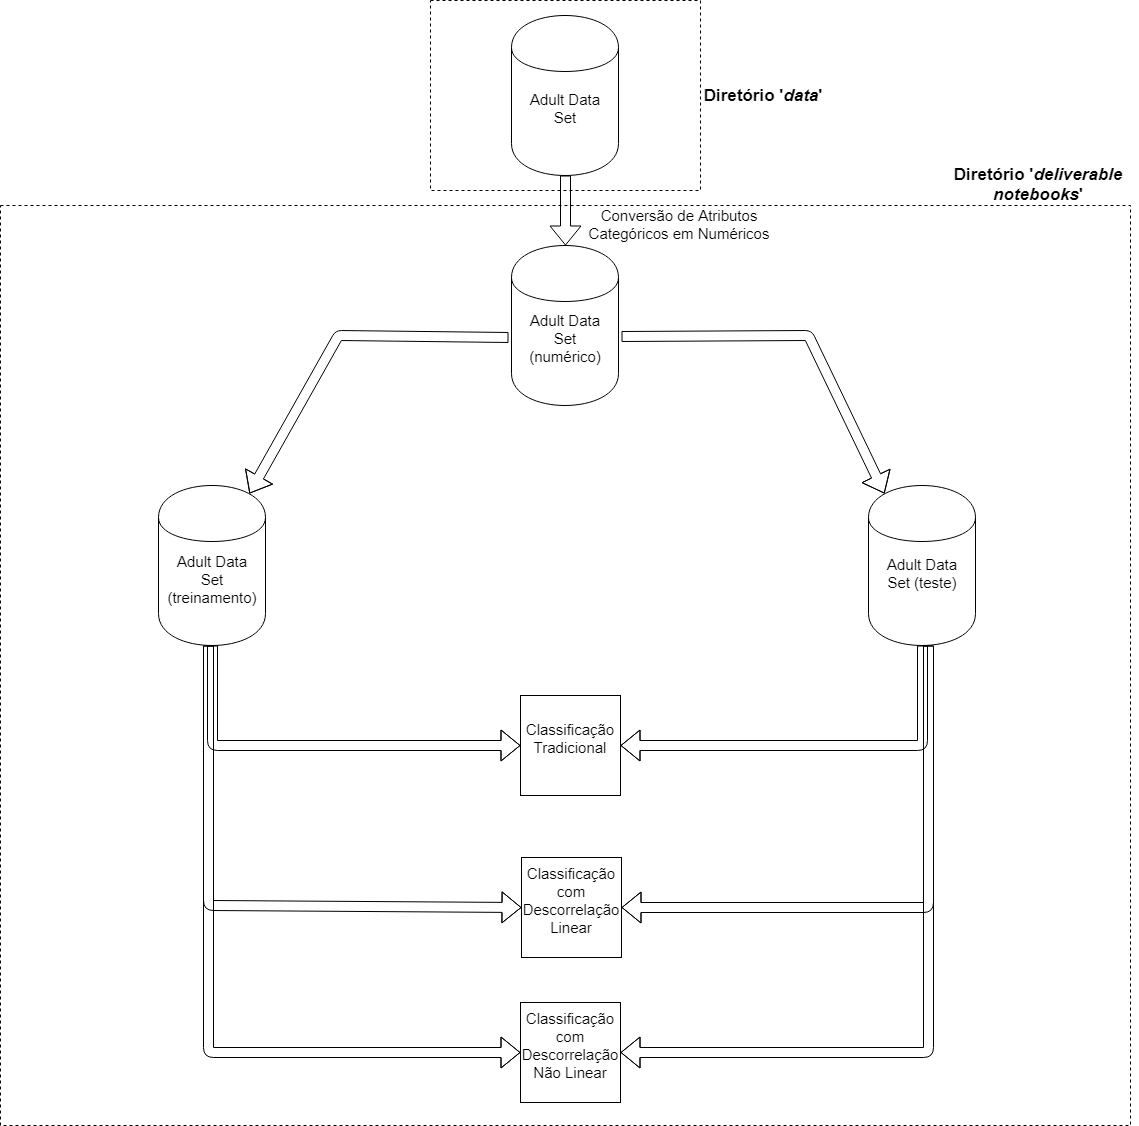
\includegraphics{../fig/WorkflowIA369.png}
\caption{Workflow}
\end{figure}

    \subsection{Resultados}\label{resultados}

Nesta seção, apresentamos nossos resultados na tarefa de classificação
em termos de acurácia e equilíbrio entre os indivíduos classificados
como "Alta Renda" nas populações masculina e feminina.

    \subsection{Classificador 1}\label{classificador-1}

Classificador baseado em regressão logística, treinado durante 5000
épocas, com os dados de treinamento originais. Para fins de comparação,
fixamos o parâmetro \emph{random-state} em 1.

    \subsection{Árvore de Decisão 1}\label{uxe1rvore-de-decisuxe3o-1}

Árvore de decisão que será comparada com o Classificador 1, também
atuando sobre os dados de treinamento originais. Fixamos o parâmetro
\emph{random-state} em 1.

    Abaixo, apresentamos a árvore de decisão para um conjunto reduzido dos
dados, para melhor visualização.
\texttt{\color{outcolor}Out[{\color{outcolor}16}]:}
    
    \begin{center}
    \adjustimage{max size={0.9\linewidth}{0.9\paperheight}}{2019-06-03-finalizacao_files/2019-06-03-finalizacao_29_0.png}
    \end{center}
    { \hspace*{\fill} \\}
    

    Para estes conjunto reduzido de dados em particular, notamos que o
atributo discriminatório não atuou na formação da árvore. Contudo, o
mesmo atributo pode ter efeitos indiretos sobre os demais, como
\emph{Workclass}, por exemplo.

    \subsection{Classificador 2}\label{classificador-2}

Classificador baseado em regressão logística, também ajustado em 5000
épocas. Para este cenário, realizamos aa descorrelação linear entre o
atributo discriminatório ("\emph{Sex}") e as classes do problema.
Novamente fixamos o parâmetro \emph{random-state} do mesmo modo que os
casos anteriores.

    \subsection{Árvore de Decisão 2}\label{uxe1rvore-de-decisuxe3o-2}

A segunda árvore de decisão treinada também atua sobre os dados
descorrelacionados, com o mesmo valor para \emph{random-state} que os
demais casos.
\texttt{\color{outcolor}Out[{\color{outcolor}19}]:}
    
    \begin{center}
    \adjustimage{max size={0.9\linewidth}{0.9\paperheight}}{2019-06-03-finalizacao_files/2019-06-03-finalizacao_35_0.png}
    \end{center}
    { \hspace*{\fill} \\}
    

    \subsection{Classificador 3}\label{classificador-3}

Finalmente, o terceiro classificador (com regressão legística) atua
sobre os dados de treinamento após realizarmos a descorrelação
não-linear entre o atributo discriminatório e as classes do problema.
Mantivemos \emph{random-state} em 1.

    \subsection{Árvore de Decisão 3}\label{uxe1rvore-de-decisuxe3o-3}

Para comparação com o classificador 3, construímos uma terceira árvore
de decisão, que também atua sobre os dados após realizarmos a
descorrelação não-linear. Também adotamos \emph{random-state=1}.
\texttt{\color{outcolor}Out[{\color{outcolor}22}]:}
    
    \begin{center}
    \adjustimage{max size={0.9\linewidth}{0.9\paperheight}}{2019-06-03-finalizacao_files/2019-06-03-finalizacao_40_0.png}
    \end{center}
    { \hspace*{\fill} \\}
    

    
    \begin{verbatim}
                    Acurácia [%]
Classificador 1            74.42
Árvore de Decisão 1        82.10
Classificador 2            75.88
Árvore de Decisão 2        81.94
Classificador 3            75.88
Árvore de Decisão 3        81.94
    \end{verbatim}

    
    Em termos de acurácia, notamos que as árvores de decisão superaram em
todos os casos os classificadores baseados em regressão logistica
associados.

Ao aplicarmos as técnicas de ICA, podemos constatar que os
classificadores 2 e 3 apresentaram uma acurácia superior ao
classificador 1. Já para o caso das árvores de decisão, notamos o
comportamento inverso: comparada com as demais, a árvore 1 apresenta a
melhor acurácia. Ainda com relação à ICA, notamos que tanto a
descorrelação linear quanto a não-linear tiveram efeitos muito parecidos
na classificação, uma vez que a acurárica do classificador 2 é igual à
do classificador 3 e o mesmo pode ser dito em relação às árvores 2 e 3.

Contudo, nosso interesse neste trabalho não é apenas com relação à
acurácia (ou outra métrica de desempenho análoga) dos classificadores.
Desejamos também avaliar a capacidade das estruturas testadas em
promover a equidade. Para tanto, na sequênca analisamos o percentutal de
indivíduos classificados como "Alta Renda" nas populações masculina e
feminina com base na classificação realizada pelas 6 estruturas
estudadas.

    
    \begin{verbatim}
                    Pop. Masc. [%] Pop. Fem. [%] Diferença [%]
Classificador 1              35.37          6.49         28.88
Árvore de Decisão 1          21.05          3.83         17.22
Classificador 2              30.33          7.26         23.08
Árvore de Decisão 2          20.89          4.29         16.61
Classificador 3              30.33          7.26         23.08
Árvore de Decisão 3          20.89          4.29         16.61
    \end{verbatim}

    
    Como primeiro resultado da tabela acima, notamos que a descorrelação
linear levou aos mesmos resultados que a descorrelação não-linear, como
podemos constatar pela igualdade dos percentuais de cada uma das
subpopulações obtidos pelos classificadores 2 e 3, assim como observamos
a igualdade entre os percentuais dos classificadores 2 e 3.

Comparando as 3 árvores de decisão, observamos que a aplicação das
técnicas de ICA levaram a um pequeno incremento na equidade, uma vez que
observamos um decréscimo de indivíduos classificados como "Alta Renda"
na população masculina e um acréscimo na mesma categoria na população
feminima. A mesma promoção de equidade notamos nos classificadores
baseados em regressão logística.

Analisando apenas a população feminina, notamos que a classificação
baseada em regressão logística levou aos maiores percentuais de "Alta
Renda". Contudo, quando analisamos as distâncias entre os pecentuais de
cada subpopulação, notamos que a menor distância ocorre para as árvores
de decisão 2 e 3.

Para o caso particular deste trabalho e da base de dados estudada, as
árvores de decisão apresentaram um melhor compromisso entre acurácia e
equidade. Também notamos que para o nosso problema, tanto a decorrelação
linear quanto a não linear levaram a resultados idênticos.

    \section{Conclusões}\label{conclusuxf5es}

Neste trabalho avaliamos como algumas das técnicas de ICA, \emph{i.e},
descorrelação linear e descorrelação não-linear, podem ser usadas para
promover a equidade na tarefa de classificação. Aplicamos estas técnicas
tanto em classificadores baseados em regressão logística quanto em
árvores de decisão. Para a base de dados que investigamos, as árvores de
decisão se mostraram mais adequadas, mantendo um bom compromisso entre
acurácia e equidade.


    % Add a bibliography block to the postdoc
    
    
    
    \end{document}
